Hoy vamos a salir de mi zona de confort y hablar sobre la creación de
\href{http://foldoc.org/macro}{\emph{macros}}, es decir, de nuevos
comandos y entornos\footnote{¡Líos de nomenclatura a la vista! Dijimos
  hace mucho que LaTeX es un \emph{conjunto de macros} para TeX. Luego
  hemos separado estas \emph{macros} en comandos y entornos, pero un
  entorno no deja de ser un conjunto de comandos que afecta de forma
  local. Llamaremos también \emph{macro} a los comandos (y por extensión
  entornos) que \emph{definamos nosotros}, tal y como se suele hacer en
  el mundillo.}. No soy ninguna experta en esto, pero hay un par de
ideas que me parece que hay que tener claras a la hora de definir cosas
en LaTeX. Básicamente voy a contar lo que me hubiera gustado que me
contaran cuando empecé con esto, más que nada para no copiar de
StackOverflow a ciegas.

Lo primero y más importante que tenemos que saber a la hora de jugar con
las macros en LaTeX es que tenemos dos opciones
\footnote{Para ser sinceros también está \lstinline!\\providecommand!, que crea el comando si no existe y si no ignora la definición, pero no tiene un\href{https://tex.stackexchange.com/questions/56667/why-is-there-no-provideenvironment}{primo para los entornos}.}:

\begin{itemize}
\item
  \textbf{Crear un entorno o comando desde cero}. Así conseguimos que
  LaTeX haga algo que no hacía o guardamos un conjunto de órdenes que
  usamos a menudo en una macro con el objetivo escribir menos. La
  palabra clave para esto es \emph{new}.
\item
  \textbf{Pisar un entorno o comando existente}. En este caso la idea es
  modificar el comportamiento de cierto comando o entorno a nuestro
  gusto. Se conoce como \emph{renew}.
\end{itemize}

El siguiente concepto en orden de importancia es que podemos (re)definir
comandos en cualquier parte del documento, pero para tener todo
perfectamente organizado es preferible hacerlo en el preámbulo.

Veamos entonces como crear comandos y entornos nuevos y modificar los
existentes. Voy a intentar que todos los ejemplos resuelvan problemas
reales, que no sean \emph{de juguete}.

\section{Escribir comandos}

Han ido apareciendo comandos nuevos\footnote{Cuando aprendimos a
  escribir
  \href{https://ondiz.github.io/cursoLatex/Contenido/05.Ecuaciones.html}{ecuaciones}
  vimos un truco para no tener que escribir la palabra \emph{Ecuación} a
  la hora de referenciar.} y trucados\footnote{Cuando hablamos del
  \href{https://ondiz.github.io/cursoLatex/Contenido/06.Idioma.html}{idioma}
  vimos cómo modificar el nombre de las tablas.} anteriormente, ¡hoy
llega por fin la explicación que os debía! Primero vamos a fabricar
comandos nuevecitos, luego modificaremos alguno que ya existe para que
sea más divertido.

\subsection{Comandos nuevos}

Definir comandos nuevos en LaTeX es sencillo, solo debemos seguir la
siguiente estructura:

\begin{lstlisting}[language={[latex]tex}]
\newcommand{COMANDO}[ARGUMENTOS]{DEFINICIÓN}
\end{lstlisting}

donde:

\begin{itemize}
\item
  \lstinline!COMANDO! será el nombre del comando que queramos definir.
  Empezará por \lstinline!\!. Solo podemos usar letras para bautizarlo.
\item
  \lstinline!ARGUMENTOS! será el número de argumentos entre 0 y 9 que le
  pasaremos al comando. Como veis, que un comando tenga argumentos es
  opcional.
\item
  \lstinline!DEFINICIÓN! será donde escribiremos lo que hace el comando.
  Haremos referencia a los diferentes argumentos mediante \lstinline!#!
  seguida del número correspondiente.
\end{itemize}

Veamos un ejemplo. Vamos a crear un comando que nos escriba
\lstinline!Figura X! en lugar de \lstinline!X! cuando hagamos referencia
a cierta figura:

\begin{lstlisting}[language={[latex]tex}]
\newcommand{\figref}[1]{\figurename~\ref{#1}}
\end{lstlisting}

Analicémoslo:

\begin{itemize}
\item
  El nombre del nuevo comando es \lstinline!\figref{}! y tiene un único
  argumento, la etiqueta de la figura, a la que hacemos referencia
  gracias a nuestro viejo conocido \lstinline!\ref{}!.
\item
  \lstinline!\figurename! es el comando que guarda el nombre de las
  figuras\footnote{\href{http://www.tex.ac.uk/FAQ-fixnam.html}{Del mismo
    modo}, el nombre de los capítulos se guarda en
    \lstinline!\\chaptername! y el de las tablas en
    \lstinline!\\tablename!. Cuidado porque no todos los elementos siguen
    este patrón, de hecho, \lstinline!\\sectionname! no existe.}.
  Podríamos escribir \emph{Figura} a mano, pero si cambiamos el idioma
  tendríamos que cambiar también la definición. De este modo LaTeX,
  sustituye \lstinline!\figurename! por el nombre de la figura según le
  mande el paquete de idioma.
\item
  Usamos un \emph{espacio duro} entre el nombre y el número para que
  LaTeX no meta en medio un salto de línea o de página.
\end{itemize}

Nuestra nueva macro se usa exactamente igual que cualquier otro comando:

\begin{lstlisting}[language={[latex]tex}]
\begin{figure}[H]
  \includegraphics[width=0.7\textwidth]{Figuras/esquema.eps}
  \caption{Esquema del proceso}
  \label{fig:esquema}
\end{figure}

Como vemos en la \figref{fig:esquema}...

% Equivalente a 
Como vemos en la Figura~\ref{fig:esquema}...
\end{lstlisting}

Un tema interesante a la hora de definir comandos es la inclusión de
\textbf{argumentos por defecto} en la definición del mismo:

\begin{lstlisting}[language={[latex]tex}]
\newcommand{COMANDO}[ARGUMENTOS][DEFECTO]{DEFINICIÓN}
\end{lstlisting}

donde \lstinline!DEFECTO! es el valor que tomará el argumento opcional
si no se especifica. El argumento opcional siempre es el primero.

Un ejemplo de uso podría ser un texto matemático en el que hagamos
referencia al plano real a menudo pero tal vez nos haga falta alguna vez
hablar de un espacio de dimensión mayor. Para ello podemos definir un
comando que nos escriba la
\href{https://en.wikipedia.org/wiki/Real_number\#/media/File:Latex_real_numbers.svg}{R
molona esa} y que por defecto el espacio sea bidimensional, pero podamos
cambiarlo opcionalmente:

\begin{lstlisting}[language={[latex]tex}]
\usepackage{amssymb}
\newcommand{\R}[1][2]{\mathbb{R}^{#1}}
\end{lstlisting}

A la hora de usarlo le pasamos el argumento opcional cuando lo
necesitamos:

\begin{lstlisting}[language={[latex]tex}]
% Espacio bidimensional
$\R$

% Espacio tridimensional
$\R[3]$
\end{lstlisting}

\subsection{Comandos trucados}

Hemos dicho al principio que además de crear nuestros propios comandos
podemos modificar el comportamiento de alguno existente. Para ello
usamos \lstinline!\renewcommand! en lugar de \lstinline!\newcommand! con
la misma sintaxis:

\begin{lstlisting}[language={[latex]tex}]
\renewcommand{COMANDO}[ARGUMENTOS]{DEFINICIÓN}
\end{lstlisting}

donde:

\begin{itemize}
\item
  \lstinline!COMANDO! será el nombre del comando que queramos modificar.
\item
  \lstinline!ARGUMENTOS! será el número de argumentos, igual que antes.
\item
  \lstinline!DEFINICIÓN! será la nueva definición del comando.
\end{itemize}

Como ejemplo de esta sección, vamos a usar \lstinline!\renewcommand!
para evitar tener que activar el modo matemático cuando escribamos
fracciones. Con este fin vamos a echar mano de
\lstinline!\ensuremath{}!,
que nos permite usar comandos matemáticos dentro y fuera de las
ecuaciones.

Como vamos a crear la nueva definición a partir del propio comando,
necesitamos guardarlo en otro sitio primero para que la definición no
sea recursiva. En este menester nos ayuda el comando
\href{https://en.wikibooks.org/wiki/TeX/let}{\lstinline!\\let!}, que
sirve para copiar el contenido de un comando en uno nuevo:

\begin{lstlisting}[language={[latex]tex}]
\let\comandoNuevo=\comandoViejo
\end{lstlisting}

Juntando las piezas, tenemos lo siguiente:

\begin{lstlisting}[language={[latex]tex}]
% Guardamos la definición original
\let\oldfrac=\frac
% Modificamos \frac para que funcione fuera de ecuaciones
\renewcommand{\frac}[2]{\ensuremath{\oldfrac{#1}{#2}}}
\end{lstlisting}

Ahora podemos usar \lstinline!\frac! directamente en el texto.

\section{Escribir entornos}

¡Ya sabemos crear y cambiar comandos! Vamos a dar un paso más y hacer
los mismo para los entornos.

\subsection{Entornos nuevos}

La sintaxis para la definición de entornos nuevos es muy similar a la de
los comandos, usando ahora \lstinline!\newenvironment!:

\begin{lstlisting}[language={[latex]tex}]
\newenvironment{ENTORNO}[ARGUMENTOS]{ANTES}{DESPUÉS}
\end{lstlisting}

En \lstinline!ANTES! escribiremos el grupo de comandos que hay que
ejecutar al iniciar el entorno y, por tanto, los que le darán el formato
al mismo, y \lstinline!DESPUÉS!, los que se activarán tras el texto. El
resto de elementos funciona como antes.

De esta manera, podemos definir un entorno para poner notas en el texto.
Yo he creado uno que rodea el texto de la nota con dos rayas
(\lstinline!\hrule!), una por debajo y una por encima, y que nos permite
darle un título, que aparecerá en negrita:

\begin{lstlisting}[language={[latex]tex}]
\newenvironment{nota}[1]
  {\vspace{1ex}\hrule\textbf{#1}}
  {\vspace{1ex}\hrule}
\end{lstlisting}

Este entorno nuevecito y reluciente se usa en el cuerpo del documento
como cualquier otro:

\begin{lstlisting}[language={[latex]tex}]
\begin{nota}{¡Cuidado!}
  Hay que tener en cuenta que
\end{nota}
\end{lstlisting}

Un tema interesante son los
\href{https://www.sharelatex.com/learn/Counters}{contadores} gracias a
los cuales podremos fabricar \textbf{entornos numerados}. Los contadores
tiene la estructura \lstinline!\theELEMENTO!. Así, \lstinline!\thepage!
contiene el número de página, \lstinline!\thechapter!\footnote{Uniéndolo
  con lo que hemos dicho anteriormente, \lstinline!\\thechapter! contiene
  el número del capítulo, \lstinline!\\chaptername! su nombre y
  \lstinline!\\chaptermark! el título.} el número de capítulo y
\lstinline!\theNOMBRE! el número del elemento numerado que hayamos
creado.

Para crear un contador usamos el comando \lstinline!\newcounter!, le
damos un nombre y, opcionalmente, le decimos dónde debe reiniciar la
cuenta:

\begin{lstlisting}[language={[latex]tex}]
\newcounter{NOMBRE}[REINICIO]
\end{lstlisting}

El tema del reinicio es interesante para los documentos largos, así
podemos empezar a contar al iniciar un capítulo y hacer referencia al
elemento mediante \lstinline!\thechapter.\theNOMBRE! que nos escribirá
el número del capítulo seguido del número del elemento. Con el ejemplo
que viene a continuación se entenderá mejor, espero.

Luego, incrementamos el valor del contador cuando sea necesario con:

\begin{itemize}
\item
  \lstinline!\stepcounter{CONTADOR}!: incrementa en uno el valor de
  \lstinline!CONTADOR!.
\item
  \lstinline!\refstepcounter{CONTADOR}!: incrementa en uno el valor de
  \lstinline!CONTADOR! y nos permite usarlo en las referencias cruzadas.
\item
  \lstinline!\addtocounter{CONTADOR}{NÚMERO}!: incrementa
  \lstinline!CONTADOR! en un valor que le pasemos.
\end{itemize}

Una idea que se me ocurre para hacer uso de esta funcionalidad es crear
un entorno numerado para poner ejemplos en el texto cuya numeración se
reinicie al cambiar de sección:

\begin{lstlisting}[language={[latex]tex}]
% Creamos un nuevo contador que se reinicie al cambiar de sección
\newcounter{ejemplo}[section]
% Incrementamos en uno el contador al iniciar el nuevo entorno
% Accedemos a su contenido con \theejemplo
\newenvironment{ejemplo}
  {\refstepcounter{ejemplo}\vspace{1ex}\hrule\textbf{Ejemplo~\thesection.\theejemplo}}
  {\vspace{1ex}\hrule}
\end{lstlisting}

Así, si escribimos algo de este estilo:

\begin{lstlisting}[language={[latex]tex}]
\section{Entorno numerado}
  \begin{ejemplo}
    Un primer ejemplo
  \end{ejemplo}

  \begin{ejemplo}
    Un segundo ejemplo
  \end{ejemplo}
\end{lstlisting}

Conseguiremos lo siguiente:

\begin{figure}[htbp]
\centering
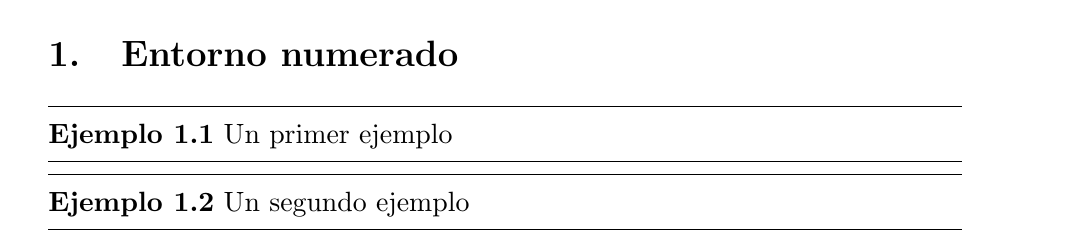
\includegraphics[width=\textwidth]{docs/Figuras/entornoNum.png}
\caption{Entornos numerados}
\end{figure}

\subsection{Entornos trucados}

Al igual que modificábamos comandos existentes con
\lstinline!\renewcommand!, podemos cambiar entornos con
\lstinline!\renewenvironment!:

\begin{lstlisting}[language={[latex]tex}]
\renewenvironment{ENTORNO}[ARGUMENTOS]{ANTES}{DESPUÉS}
\end{lstlisting}

Lo que tenemos que tener en cuenta aquí es la implementación original
del entorno que vamos a cambiar. A mí me ayuda pensar en un entorno como
dos comandos, uno que da inicio al formato concreto y otro que lo
finaliza. Es decir, esto:

\begin{lstlisting}[language={[latex]tex}]
\begin{equation}
  a^2 x + b x + c = 0
\end{equation}
\end{lstlisting}

es equivalente a:

\begin{lstlisting}[language={[latex]tex}]
\equation
  a^2 x + b x + c = 0
\endequation
\end{lstlisting}

De esta manera me resulta más sencillo saber qué hay que escribir en los
argumentos \lstinline!ANTES! y \lstinline!DESPUÉS! de los que hablaba.

Para terminar con los entornos os dejo con un ejemplo complejo que monté
juntando piezas de aquí y de allí para que las citas aparecieran en gris
oscuro con una barrita gris clara a la izquierda. Es complicadillo y yo
misma no sé si lo entiendo muy bien, pero es para que veáis un caso
real:

\begin{lstlisting}[language={[latex]tex}]
\usepackage{framed}

% Redefinir leftbar
\renewenvironment{leftbar}[1][\hsize]
  {\color{gray}
    \def\FrameCommand
    {{\color{lightgray}\vrule width 3pt}}
    \MakeFramed{\hsize#1\advance\hsize-\width\FrameRestore}
  }
  {\endMakeFramed}
  
% Guardar entorno quote, lo forman dos comandos
\let\oldquote=\quote
\let\oldendquote=\endquote

% Barra vertical a la izquierda de la cita
\renewenvironment{quote}
  {\vspace{10pt}\leftbar\vspace*{-6pt}\oldquote}
  {\oldendquote\endleftbar\vspace{10pt}}
\end{lstlisting}

En fin, creo que la única manera de aprender a modificar entornos es
modificar entornos así que no queda más remedio que practicar.

\section{Una nota sobre TeX}

En el principio de los tiempos dijimos que LaTeX es un conjunto de
macros escritos en TeX (o Plain TeX) ¿recordáis? Esto provoca que LaTeX
tenga algunas limitaciones a la hora de definir cosas, limitaciones que
TeX, al ser de más bajo nivel, no tiene.

El comando \lstinline!\let! que hemos usado para guardar la definición
original de un comando que íbamos a modificar pertenece a TeX. También
\lstinline!\def! que
aparece en ejemplo de las citas personalizadas es parte de TeX y sirve
para definir comandos nuevos, al igual que
\lstinline!\newcommand!\footnote{Se pueden declarar comandos nuevos
  dentro de entornos de manera similar a declararlos de manera
  independiente.
  \href{https://en.wikibooks.org/wiki/LaTeX/Macros\#Declare_commands_within_new_environment}{Aquí}
  tenéis más información.}. Os hablo de ellos porque los veréis a menudo
cuando busquéis ejemplos por ahí.

\section{En definitiva, ¿qué hay que
saber?}

Diría que lo más importante es saber la diferencia entre \emph{definir}
(\lstinline!\new!) y \emph{pisar} (\lstinline!\renew!) un comando o
entorno existente y cuándo hay que hacer lo uno o lo otro. Tampoco está
de más recordar que escribimos tanto las definiciones como las
modificaciones en el preámbulo. Igualmente, nos viene bien saber de la
existencia de comandos de TeX como \lstinline!\let! y \lstinline!\def!
que nos hacen la vida más fácil.

Para acabar, os dejo mi proceso para crear macros:

\begin{enumerate}
\def\labelenumi{\arabic{enumi}.}
\item
  Escribo mi combinación de comandos en el cuerpo del documento y
  verifico que funciona.
\item
  Escribo cómo quiero que sea mi comando o entorno final y lo comparo
  con mi combinación de comandos.
\item
  Traslado la combinación al preámbulo y le doy forma según la sintaxis
  correspondiente.
\item
  Extraigo los argumentos y pienso si puedo darle un valor por defecto a
  alguno de ellos.
\item
  Pruebo si funciona.
\end{enumerate}

Lo dicho, a escribir macros se aprende escribiendo macros. ¡Dadle duro!

\section{Referencias}\label{referencias}

\href{http://alvinalexander.com/blog/post/latex/create-your-own-commands-in-latex-using-newcommand}{\emph{LaTeX
example: How to create your own commands with \lstinline!newcommand!}}

\href{https://en.wikibooks.org/wiki/LaTeX/Macros}{\emph{LaTeX/Macros} en
Wikibooks}

\href{http://www.shawnlankton.com/2008/01/newcommand-with-argument-in-latex/}{\emph{\\newcommand
with arguments in LaTeX}}

\href{https://tex.stackexchange.com/questions/35564/plain-tex-vs-latex-macros}{\emph{Plain
TeX vs.~LaTeX Macros} en TeXExchange}

\href{https://en.wikibooks.org/wiki/LaTeX/Plain_TeX}{\emph{LaTeX/Plain
TeX} en Wikibooks}

\href{https://tex.stackexchange.com/questions/26742/list-of-higher-level-latex-commands-corresponding-to-tex-commands/26922\#26922}{\emph{List
of higher-level LaTeX commands corresponding to TeX commands} en
TeXExchange}

\href{https://tex.stackexchange.com/questions/655/what-is-the-difference-between-def-and-newcommand}{\emph{What
is the difference between \\def and \\newcommand?} en TeXExchange}
